\documentclass[12pt, letterpaper, twoside]{report}
\usepackage[utf8]{inputenc}
\usepackage{graphicx}
\usepackage{verbatim}
\graphicspath{{images/}}
\usepackage{url}

\title{\textbf{htmldate}}
\author{Abdulqudus Olayinka Awesu}
\date{2020 August 06}

\begin{document}

\maketitle

% \begin{abstract}
  
%  \end{abstract}

\chapter{Introduction}
Nowadays, we have lots of data moving around the globe, making data extraction clumsy, but with the inclusion of dates, web content is analyzed easily. Having an adequate and updated report is crucial in the area of research and publication, which can minimize the issues caused by the information explosion. When researchers have high levels of expertise, social interactions provide them with more precious insights than reading journal papers, and they value discussions with peers for keeping up to date. htmldate is a python package that scans throgh the web for original and updated web articles and blogs date. htmldate make use of module call finddate to scan through for dates on web pages 

\section{What is the problem?}
We would like to know how often information are been updated on \textit{MIT-News} concerning machine learning article or blogs, for better clarification htmldate was used.  

\section{Data source}
we have used the \textit{MIT-News} data for a clarification of our trend on machine learning  

 \url{http://news.mit.edu/topic/machine-learning?page=1}

\section{Description of workflow}
\begin{itemize}
  \item we Imported htmldate modules, numpy, pandas, matplotlib.pyplot, ipywidget, interact, csv,
  \item We used ipywidget to beautify the notebook 
  \item The list was saved into a csv file.
  \item we used widget to design the drop down list.
  \item we used widget and wrote a function to select each web link to display the publication date
  \item We used matplotlib to plot the trends of how often articles are posted.
  \item Used LaTex to create report PDF.
  \item We Created a Makefile for the automation of this project.
\end{itemize}

\chapter{Graphs}
 

\section{matplotlib Garaph}
 PLOT SHOWING PUBLICATION DATES OF DIFFERENT WEB ARTICLES
\begin{figure}[ht]
    \centering
    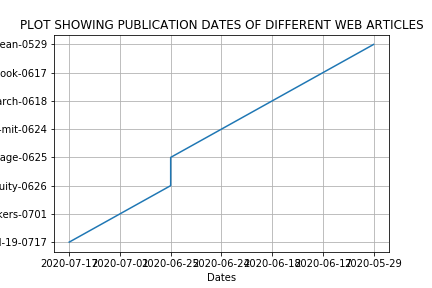
\includegraphics[width=0.8\textwidth]{test.png}
    \caption{ Publication dates of different web articles}
    \label{fig:Trends}
\end{figure}

 \chapter{htmldate Reports}
%  \verbatiminput{Report.txt}
htmldate has not been able to perfect the extraction of publication dates from web links without a guessing.
The table below shows the documentation of Python packages similar to htmldate
\section{Analysis of htmldate }

\begin{figure}[ht]
    \centering
    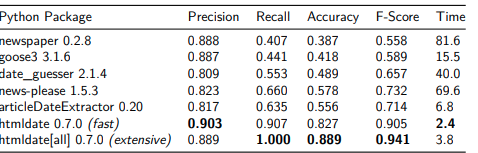
\includegraphics[width=0.8\textwidth]{table.png}
    \caption{Result of htmldate in comparison with its alternative}
    \label{fig:Table}
\end{figure}
 
@article{Barbaresi2020,
  DOI = {10.21105/joss.02439},
  url = {\url{https://doi.org/10.21105/joss.02439}},
  year = {2020},
  publisher = {The Open Journal},
  volume = {5},
  number = {51},
  pages = {2439},
  author = {Adrien Barbaresi},
  title = {htmldate: A Python package to extract publication dates
from web pages},
  journal = {Journal of Open Source Software}
}

 \end{document}